\documentclass{article}
\usepackage[T2A]{fontenc}
\usepackage[serbianc]{babel}
\usepackage{graphicx}
\usepackage{subcaption}
\usepackage[obeyspaces]{url}
\usepackage[margin=1.0in, top=0.5in]{geometry}
\usepackage{amsmath}
\usepackage{listings}
\usepackage{color}
\usepackage[utf8]{inputenc}
\usepackage{listingsutf8}
\usepackage[absolute,overlay]{textpos}

\begin{document}
\begin{titlepage}
    \begin{textblock*}{10cm}(1cm,1cm)
        \textbf{\hspace{-0.779cm}  Универзитет у Новом Саду\\Факултет техничких наука\\Нови Сад}
    \end{textblock*}

    \begin{textblock*}{10cm}(1cm,24.38cm)
        \textbf{\hspace{-0.779cm} Департман за рачунарство\\и аутоматику\\Одсек за рачунарску технику\\и рачунарске комуникације}
    \end{textblock*}

    \begin{textblock*}{10cm}(10.5cm,1cm)
        \raggedleft
        \textbf{\today}
    \end{textblock*}
    
    \null\vspace{\stretch{0.3}}
    
    \begin{center}
        \textbf{\LARGE Пројектни задатак}
        
        \vspace{1.5cm}
        
        \textbf{\large Немања Милошевић RA 200/2021}\\
        \vspace{0.15cm}
        \textbf{\large Вук Михаљчић RA 218/2021}\\
        \vspace{0.15cm}
        \textbf{\large Алекса Станковић RA 219/2021}\\
 	 \vspace{0.15cm}
        \textbf{\large Марко Пушковић RA 230/2021}
        
        \vspace{3.5cm}
        \textbf{\Huge Framebuffer + Sega GPU}\\
        \vspace{0.5cm}
        \textbf{\large Логичко пројектовање рачунарских система 2}
        
        \vfill
        
        \begin{flushright}
            \textbf{\large Ментори:}\\
            \textbf{др Милош Суботић}\\
            \textbf{проф. др Иван Каштелан}
        \end{flushright}
    \end{center}
\end{titlepage}




\section{Задатак}
Задатак пројекта у склопу предмета ЛПРС2 је дизајнирање игре по угледу на игре SEGA играчке конзоле. У овом случају имплементирана је игра случна игри Pong користећи језик VHDL за пројектовање, FPGA плочицу на којој ће она извршавати и N64 играчки контролер којим ће се управљати играчима.\par

Документација обухвата процес развијања игре, њене спецификације и дизајн.

\section{Преглед игре}
Игра се састоји од двају играча у виду танких црних рекета, крећућих се вертикално, и црне лоптице на белој позадини. Резултат се бележи помоћу квадратићâ зелене и плаве боје за левог и десног играча, респективно.\par
Када лоптица прође иза играча, противник осваја бод. Победник је играч освојивши 5 бодова у току партије.
 

\section{Спецификације дизајна}
Систем развијања игре обухвата један рачунар у којем је писан VHDL код игре, додатни монитор на којем се прати одвијање игре, N64 контролер и FPGA плочицу.
\subsection{Архитектура система}
Цели систем заснива се на FPGA плочици. Она је компонента која извршава програм и повезује остали хардвер.

\subsubsection{Графичка спрега система}
FPGA уређај комуницира с монитором шаљући сигнале путем HDMI везе. Резолуција излаза је 640x480 пиксела и ради на такту освежавања од 60 Hz.

\subsubsection{Протокол за комуникацију с контролером}
Протокол је заснован на обостраној комуникацији између FPGA система (водећи, енг. master) и контролера (пратећи, енг. slave). При комуникацији водећи шаље 9-битну поруку 0b000000001 којом затражује од пратећега повратну информацију о стању тастерâ, величине 34 бита.

% овде слика
	\begin{figure}[h]
	    \centering
	    \includegraphics[width=0.15\textwidth]{N64.png}
	    \caption{Формат одговора}
	    \label{fig:your_label}
	\end{figure}
\newpage
\subsubsection{Комуникација хардверских компоненти}
Радни такт износи 50 Hz. Логичке цифре (0 и 1) састоје се од 200 периода такта. Нулу чине првих 150 периода на ниском напонском нивоу и затим 50 периода на високом. Јединицу чине 50 нисконапонских и 150 високонапонских периода.
\begin{figure}[h]
    \centering
    \begin{subfigure}[b]{0.4\textwidth}
        \centering
        \includegraphics[width=\textwidth]{zero64.png}
        \caption{Логичка нула}
        \label{fig:subfig1}
    \end{subfigure}
    \hfill
    \begin{subfigure}[b]{0.4\textwidth}
        \centering
        \includegraphics[width=\textwidth]{one64.png}
        \caption{Логичка јединица}
        \label{fig:subfig2}
    \end{subfigure}
    \caption{Логичке цифре у комуникацији}
    \label{fig:fig}
\end{figure}\par
% оне две слике

\subsubsection{Аутомат коначног броја стања за комуникацију с водеће стране}
Стања се могу представити аутоматом:
\begin{itemize}
	\item IDLE\_FSM - систем чека да се активира
	\item POLL\_FSM - FPGA шаље конторлеру захтев од 9 битова
	\item SEND0\_FSM1 - слање првог дела логичке нуле
	\item SEND0\_FSM2 - слање другог дела логичке нуле
	\item SEND1\_FSM1 - слање првог дела логичке јединице
	\item SEND1\_FSM2 - слање другог дела логичке јединице
	\item GET\_FSM - почетак примања одговора од контролера
	\item FINISH\_FSM - складиштење стања тастерâ контролера
\end{itemize}
% слика аутомата
\newpage
\begin{figure}[h]
    \centering
    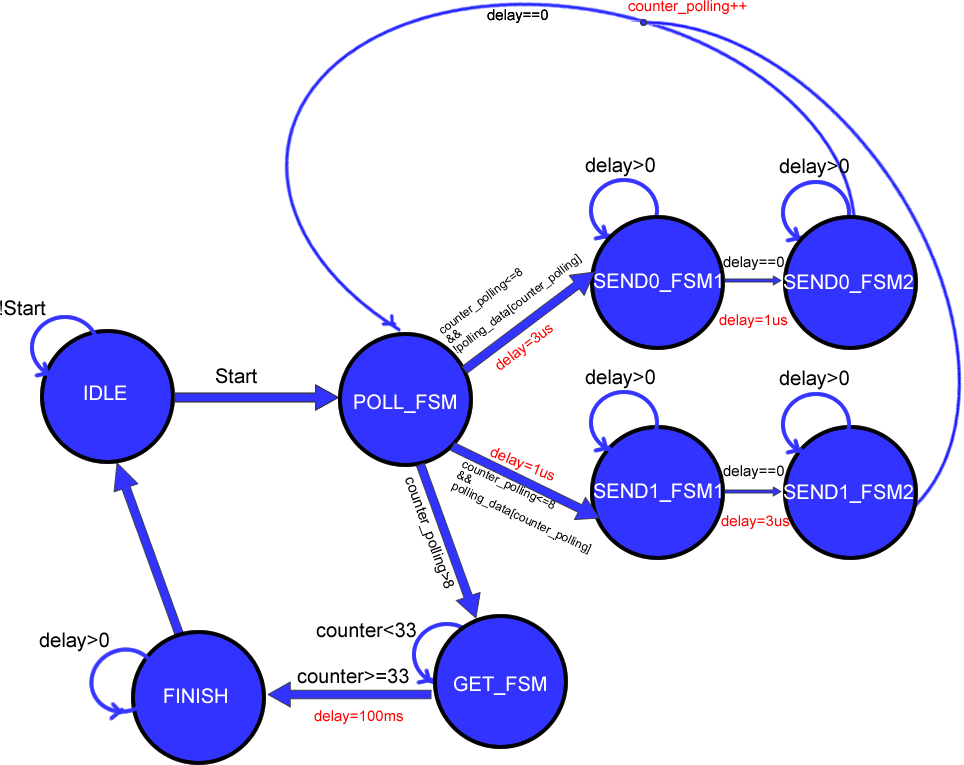
\includegraphics[width=0.8\textwidth]{FSM_Diagram.png}
    \caption{Аутомат}
    \label{fig:your_label}
\end{figure}


\subsection{Програмска подршка}
Логика игре је имплементирана у језику за опис хардвера VHDL. Софтверска решења игре и контролера су одвојени модули, тако да су међусобно независни. Датотеке игре се налазе у директоријуму\path{ LPRS2_2024/FB_Sega_GPU/FPGA/LPRS2_HDMI_Cam_N64_Joypad_LED}.\par
Програмска подршка управља стањем целокупне игре: 
\begin{itemize}
\item физика (судари, кретање лопте и играчâ)
\item праћење тренутног резултата
\item обрада улаза периферије
\item приказ на екран (енг. render)
\end{itemize}

\subsubsection{Физика}
Лопта и играчи имају сопствене брзине кретања. Током свакога фрејма приказа положај ентитетâ се обнавља у односу на њихову брзину. Ако лопта удари у горњу или доњу ивицу екрана, њена вертикална брзина се инвертује. Ако играчи ударе у хоризонталне ивице, бивају заустављени, како не би изашли из визуелног опсега. Ако лопта удари у једног од играча, одбија се од њега према противничкому играчу. Уколико играч не успе одбити лопту, лопта излази из опсега прошавши вертикалну ивицу, те се противнику додељује бод.

\subsubsection{Праћење тренутног резултата}
Када је играчу додељен бод, лопта се поново изводи на средину поља и бод се бележи у извесној променљивој. Када вредност бодова достигне 5, игра се враћа у почетно стање и меч почиње изнова.

\subsubsection{Обрада улаза периферије}
На контролеру постоје 4 релевантна тастера: UP, DOWN, C\_UP, C\_DOWN.\par
Први играч се покреће помоћу првих двају тастера, а други помоћу других. У случају истовременог притиска на горњи и доњи тастер, играч се неће померити.

\subsubsection{Приказ на екран}
Постоје 3 групе објеката приказивања:
\begin{itemize}
\item играчи - представљени су у облику танких правоугаоника црне боје
\item лопта - представљена је у облику малог квадрата црне боје
\item резултат - представљен је у горњем делу екрана у виду зелених и плавих квадратића
\end{itemize}

\section{Компилација и покретање игре}
Ради компилације користи се програмско окружење Intel Quartus 8.0. Најпре код мора проћи кроз анализу и синтезу; то се постиже пречицом Ctrl + L. Након тога процес компилације се завршава и потом је потребно отворити Programmer, чија је улога „спуштање“ кода на FPGA плочицу. Игру покренити кликом на Start.








% Your content goes here


\end{document}